\documentclass[10pt]{article}

\usepackage{graphicx,color,epsfig}
\newcommand{\manualpath}{.}
\newcommand{\inputslocation}{\manualpath/inputs/}
\graphicspath{{\manualpath/diagrams/}{\manualpath/screencaps/}}

	
\usepackage{listings}
\lstset{language=}
\renewcommand\lstlistingname{File}
\renewcommand\lstlistlistingname{Files}
\lstset{numbers=none, numberstyle=\tiny, stepnumber=1, numbersep=5pt,captionpos=b,frame=single,breaklines=true,basicstyle=\small}




	
\usepackage{amsgen,amsmath,amstext,amsbsy,amsopn,amssymb}

\usepackage[dvipsnames]{xcolor}

\usepackage[colorlinks]{hyperref}
\hypersetup{
    colorlinks=true,       % false: boxed links; true: colored links
    linkcolor=Plum,          % color of internal links (change box color with linkbordercolor)
    citecolor=green,        % color of links to bibliography
    filecolor=magenta,      % color of file links
    urlcolor=cyan           % color of external links
}


\usepackage{float}

\usepackage[english]{babel}

\usepackage[left=1.25in,right=1.25in,top=1.25in,bottom=1.25in]{geometry} %
\usepackage[singlespacing]{setspace}%line spacing, set default to double

\usepackage{array}



\usepackage{makeidx}
\makeindex
	
	
\usepackage[format=plain,indention=.5cm,margin=10pt,font={small,singlespacing}]{caption}%custom captions.
\setlength{\parskip}{1em} %custom spacing between paragraphs 
	
	
	



% Alter some LaTeX defaults for better treatment of figures:
% See p.105 of "TeX Unbound" for suggested values.
% See pp. 199-200 of Lamport's "LaTeX" book for details.
%   General parameters, for ALL pages:
\renewcommand{\topfraction}{0.9}	% max fraction of floats at top
\renewcommand{\bottomfraction}{0.8}	% max fraction of floats at bottom
%   Parameters for TEXT pages (not float pages):
\setcounter{topnumber}{2}
\setcounter{bottomnumber}{2}
\setcounter{totalnumber}{4}     % 2 may work better
\setcounter{dbltopnumber}{2}    % for 2-column pages
\renewcommand{\dbltopfraction}{0.9}	% fit big float above 2-col. text
\renewcommand{\textfraction}{0.07}	% allow minimal text w. figs
%   Parameters for FLOAT pages (not text pages):
\renewcommand{\floatpagefraction}{0.7}	% require fuller float pages
% N.B.: floatpagefraction MUST be less than topfraction !!
\renewcommand{\dblfloatpagefraction}{0.7}	% require fuller float pages

% remember to use [htp] or [htpb] for placement

 

%scaling for the screen caps used in the manual
\newcommand{\screencapsize}{0.41}

%for inputting paramotopy input files
\newcommand{\File}[3]{
\begin{center}

\begin{minipage}{0.8\linewidth}
\lstinputlisting[
	caption={#1},
	label=file:#2]{\inputslocation#3}
\end{minipage}

\end{center}
}


%for inputting bertini real input files
\newcommand{\Filenobox}[3]{

\lstinputlisting[frame=none,
	breaklines=true,
	caption={#1},
	label=#2]{\inputslocation#3}

}

\usepackage{marginnote}
\renewcommand*{\marginfont}{\color{red}\sffamily\tiny}
\newcommand{\comment}[1]{\textcolor{red}{$\star$}\marginnote{#1}}



\usepackage[utf8]{inputenc}



\usepackage[acronym,toc,xindy]{glossaries}
\makeglossaries
\newglossaryentry{cmap}
{
    name=colormap,
    description={The set of colors that are used to vivify a figure in MATLAB},
    plural=colormaps
}
 
\newglossaryentry{dependent}
{
    name=dependency,
    description={A program (or programs) that need(s) to be installed in order for a different program to run},
    plural=dependencies
}
 
\newglossaryentry{rgbt} {
  name={RGB triple},
  description={A row vector with three columns with each entry ranging from zero to one used to identify a color},
  plural=RGB triples
}

\newglossaryentry{cpath}
{
    name=CPATH,
    description={A list of directories to be automatically searched for libraries, but are searched after all libraries tagged with \-I}
}

\newglossaryentry{lib}
{
    name=LIBRARY\_PATH,
    description={The value of LIBRARY\_PATH is a colon-separated list of directories, much like PATH. When configured as a native compiler, GCC tries the directories thus specified when searching for special linker files}
}
 
\newglossaryentry{ldlib}
{
    name=LD\_LIBRARY\_PATH,
    description={LD is the name of the unix linker. This environment variable is a colon-separated set of directories where libraries should be searched for first, before the standard set of directories and is useful when debugging a new library or using a nonstandard library for special purposes.}
} 

\newglossaryentry{path}
{
    name=PATH,
    description={The PATH environment variable is used by Cygwin applications as a list of directories to search for executable files to run.}
}

\newacronym[see={[Glossary:]{rgbt}}]{RGB}{RGB}{Red Green Blue color values\glsadd{rgbt}}

\newacronym{mpi}{MPI}{Message Passing Interface}

\newacronym{gmp}{GMP}{GNU Multiple Precision Arithmetic Library}

\newacronym{gcc}{GCC}{GNU C Compiler}

\newacronym{mpfr}{MPFR}{Multiple Precision Floating-Point Reliable}

\newacronym{mpc}{MPC}{GNU Multiple Precision Complex Library}

\newacronym{stl}{STL}{stereolithography}



\usepackage{multirow, bigstrut, booktabs}
\usepackage{longtable}
\usepackage{tabu}


\usepackage{titlesec}
\newcommand{\sectionbreak}{\clearpage}




\usepackage{graphicx}

\begin{document}
\pagestyle{plain} 
	\pagenumbering{roman} 
	\setcounter{page}{1}




\thispagestyle{empty}


\begin{center}


\quad % put in a space so the following vspace command succeeds
\vspace{3in}


{\LARGE Bertini\_Real}\\[\baselineskip]
User's Manual
\vskip0.5in
\comment{need a sweet picture here}

\vfill%\vskip2in
%\includegraphics[width = 0.55\linewidth]{}

\end{center}
\null
\vfill
\begin{singlespace}
Manual by\\
Pierce Cunneen \& Daniel Brake\\
University of Notre Dame \\
ACMS \hfill \today
\end{singlespace}
\newpage





	\tableofcontents
	\eject
	\pagenumbering{arabic} 
	\setcounter{page}{1}
	\eject



\section{Introduction}


Welcome to Bertini\_real, software for real algebraic geometry.  This manual is intended to help the user operate this piece of numerical software, to obtain useful and high-quality results from decomposing real algebraic curves and surfaces.

Bertini\_real is compiled software, links against a parallel version of Bertini 1 compiled as a library, and requires Matlab and the Symbolic Computation toolbox.  It also requires several other libraries, including a few from Boost, and an installation of MPI.  All libraries should be compiled using the same compilers.  

\subsection{Contact}
\label{sec:contact}

\subsection*{Acknowledgements}
\begin{itemize}
\item  This research utilized the CSU ISTeC Cray HPC System supported by NSF Grant CNS-0923386.
\item  This material is based upon work supported by the National Science Foundation under Grants No. DMS-1025564 and DMS-1115668.
\end{itemize}

\subsection{License}
\label{sec:license}

\subsection*{Disclaimer}

Any opinions, findings, and conclusions or recommendations expressed in this material are those of the author(s) and do not necessarily reflect the views of the National Science Foundation or any other organization.




\clearpage
\section{Quick Start}
\label{sec:started}

Bertini\_real can be downloaded from \url{http://bertinireal.com/download.html}. Use of Bertini\_real depends on Bertini, which itself has several important dependencies (see section \ref{sec:installation})
Once installed, you can run Bertini\_real on an input file from the command line. After navigating to the working directory of the input file, the flow of Bertini\_real is as follows:
\begin{enumerate}
\item Run Bertini on an input file using the \texttt{tracktype:1} setting. This is done by typing in the command line: \texttt{bertini} with an input file named \texttt{input}. Bertini will produce a Numerical Irreducible Decomposition that will be used by Bertini\_real.
\item Run Bertini\_real on the same input file. Similarly, just type \texttt{bertini\_real} in the command line. Bertini\_real will provide a cellular decomposition of the real portion of a one- or two- dimensional complex algebraic set.
\item Visualize the results of Bertini\_real in MATLAB. Enter MATLAB and call \texttt{gather\_br\_samples}, which parses the output results of  into a .mat file, and then call \texttt{bertini\_real\_plotter}, which will plot the curve or surface in MATLAB (N.B. The MATLAB executable must be on the path to the input file for Bertini\_real to run). 
\end{enumerate}

\subsection{A Quick Example: The Cayley Cubic}
This section will outline the steps to running Bertini, Bertini\_real, and finally visualizing the Cayley Cubic, an interesting 3D surface. The first step is to create an input file. Open up a text editor and create a file called \texttt{input}. 
Below is the text for this input file.. A key feature to notice is the second line, where the \texttt{tracktype} configuration is set to 1. This configuration setting is necessary for Bertini\_real to run.  \newline \newline
\texttt{CONFIG \newline
tracktype:1;\newline
imagthreshold:1e-5;\newline
END;\newline
INPUT\newline
variable\_group x, y, z;\newline
function f;\newline
$f = 4 * (x^2 + y^2 + z^2) + 16*x*y*z - 1$;\newline
END; \newline}
\clearpage
Once the input file is created, running Bertini is simple. Simply navigate in the command line to the directory of the input file and type \texttt{bertini}. This will run Bertini, creating the Numerical Irreducible Decomposition needed for Bertini\_real. The following should print to terminal/shell: \par
\begin{figure}[!hb]
	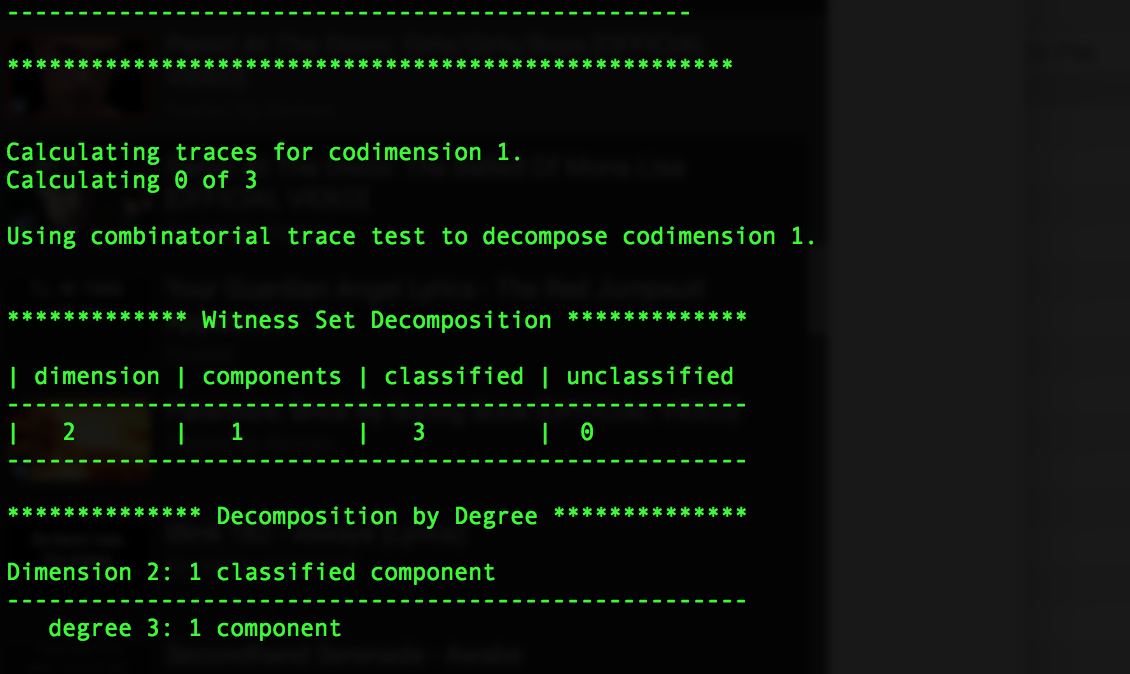
\includegraphics[width = 11cm, height = 5cm]{CayleyCubicBertiniRun.png}
\end{figure}


Once Bertini is finished, the output can be verified as satisfactory. Then, Bertini\_real can be run by calling \texttt{bertini\_real} in the command line. This should take roughly 20-30 seconds, with the final terminal/shell output appearing below:
\begin{figure}[!hb]
	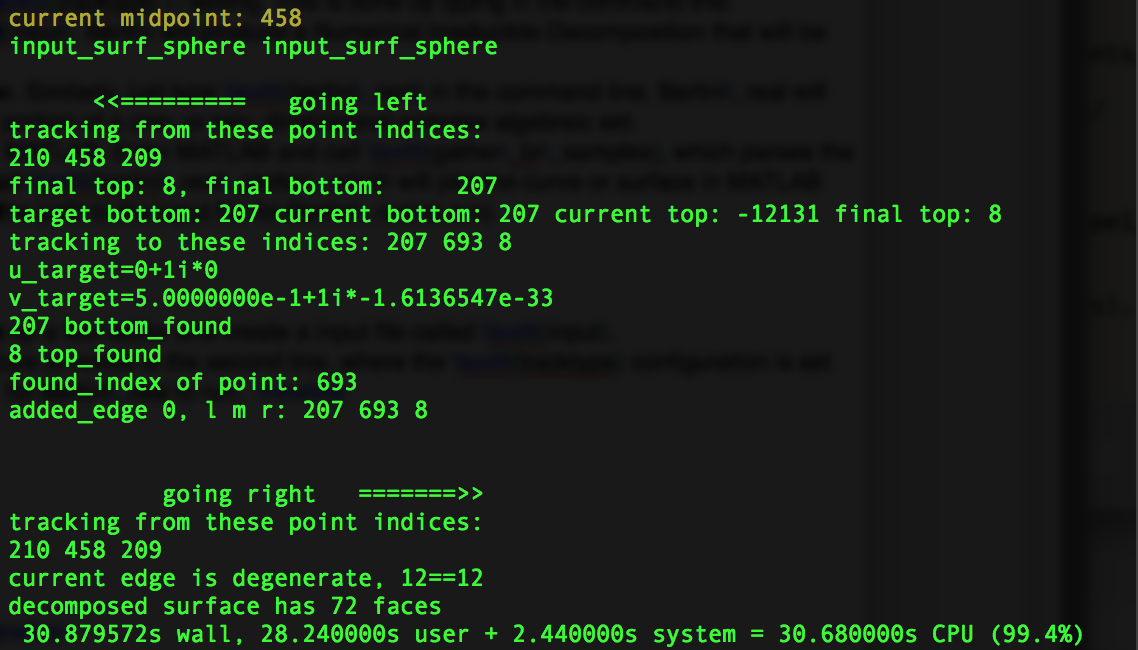
\includegraphics[width = 11cm, height = 5cm]{CayleyCubicBertiniRealRun.png}
\end{figure}

Finally, MATLAB can be used to visualize the result from the Bertini\_real run. Open MATLAB and call \texttt{gather\_br\_samples}, which generates a .mat file. Then, call \texttt{bertini\_real\_plotter}. This will create a MATLAB figure, pictured below. 

\begin{figure}[!hb]
	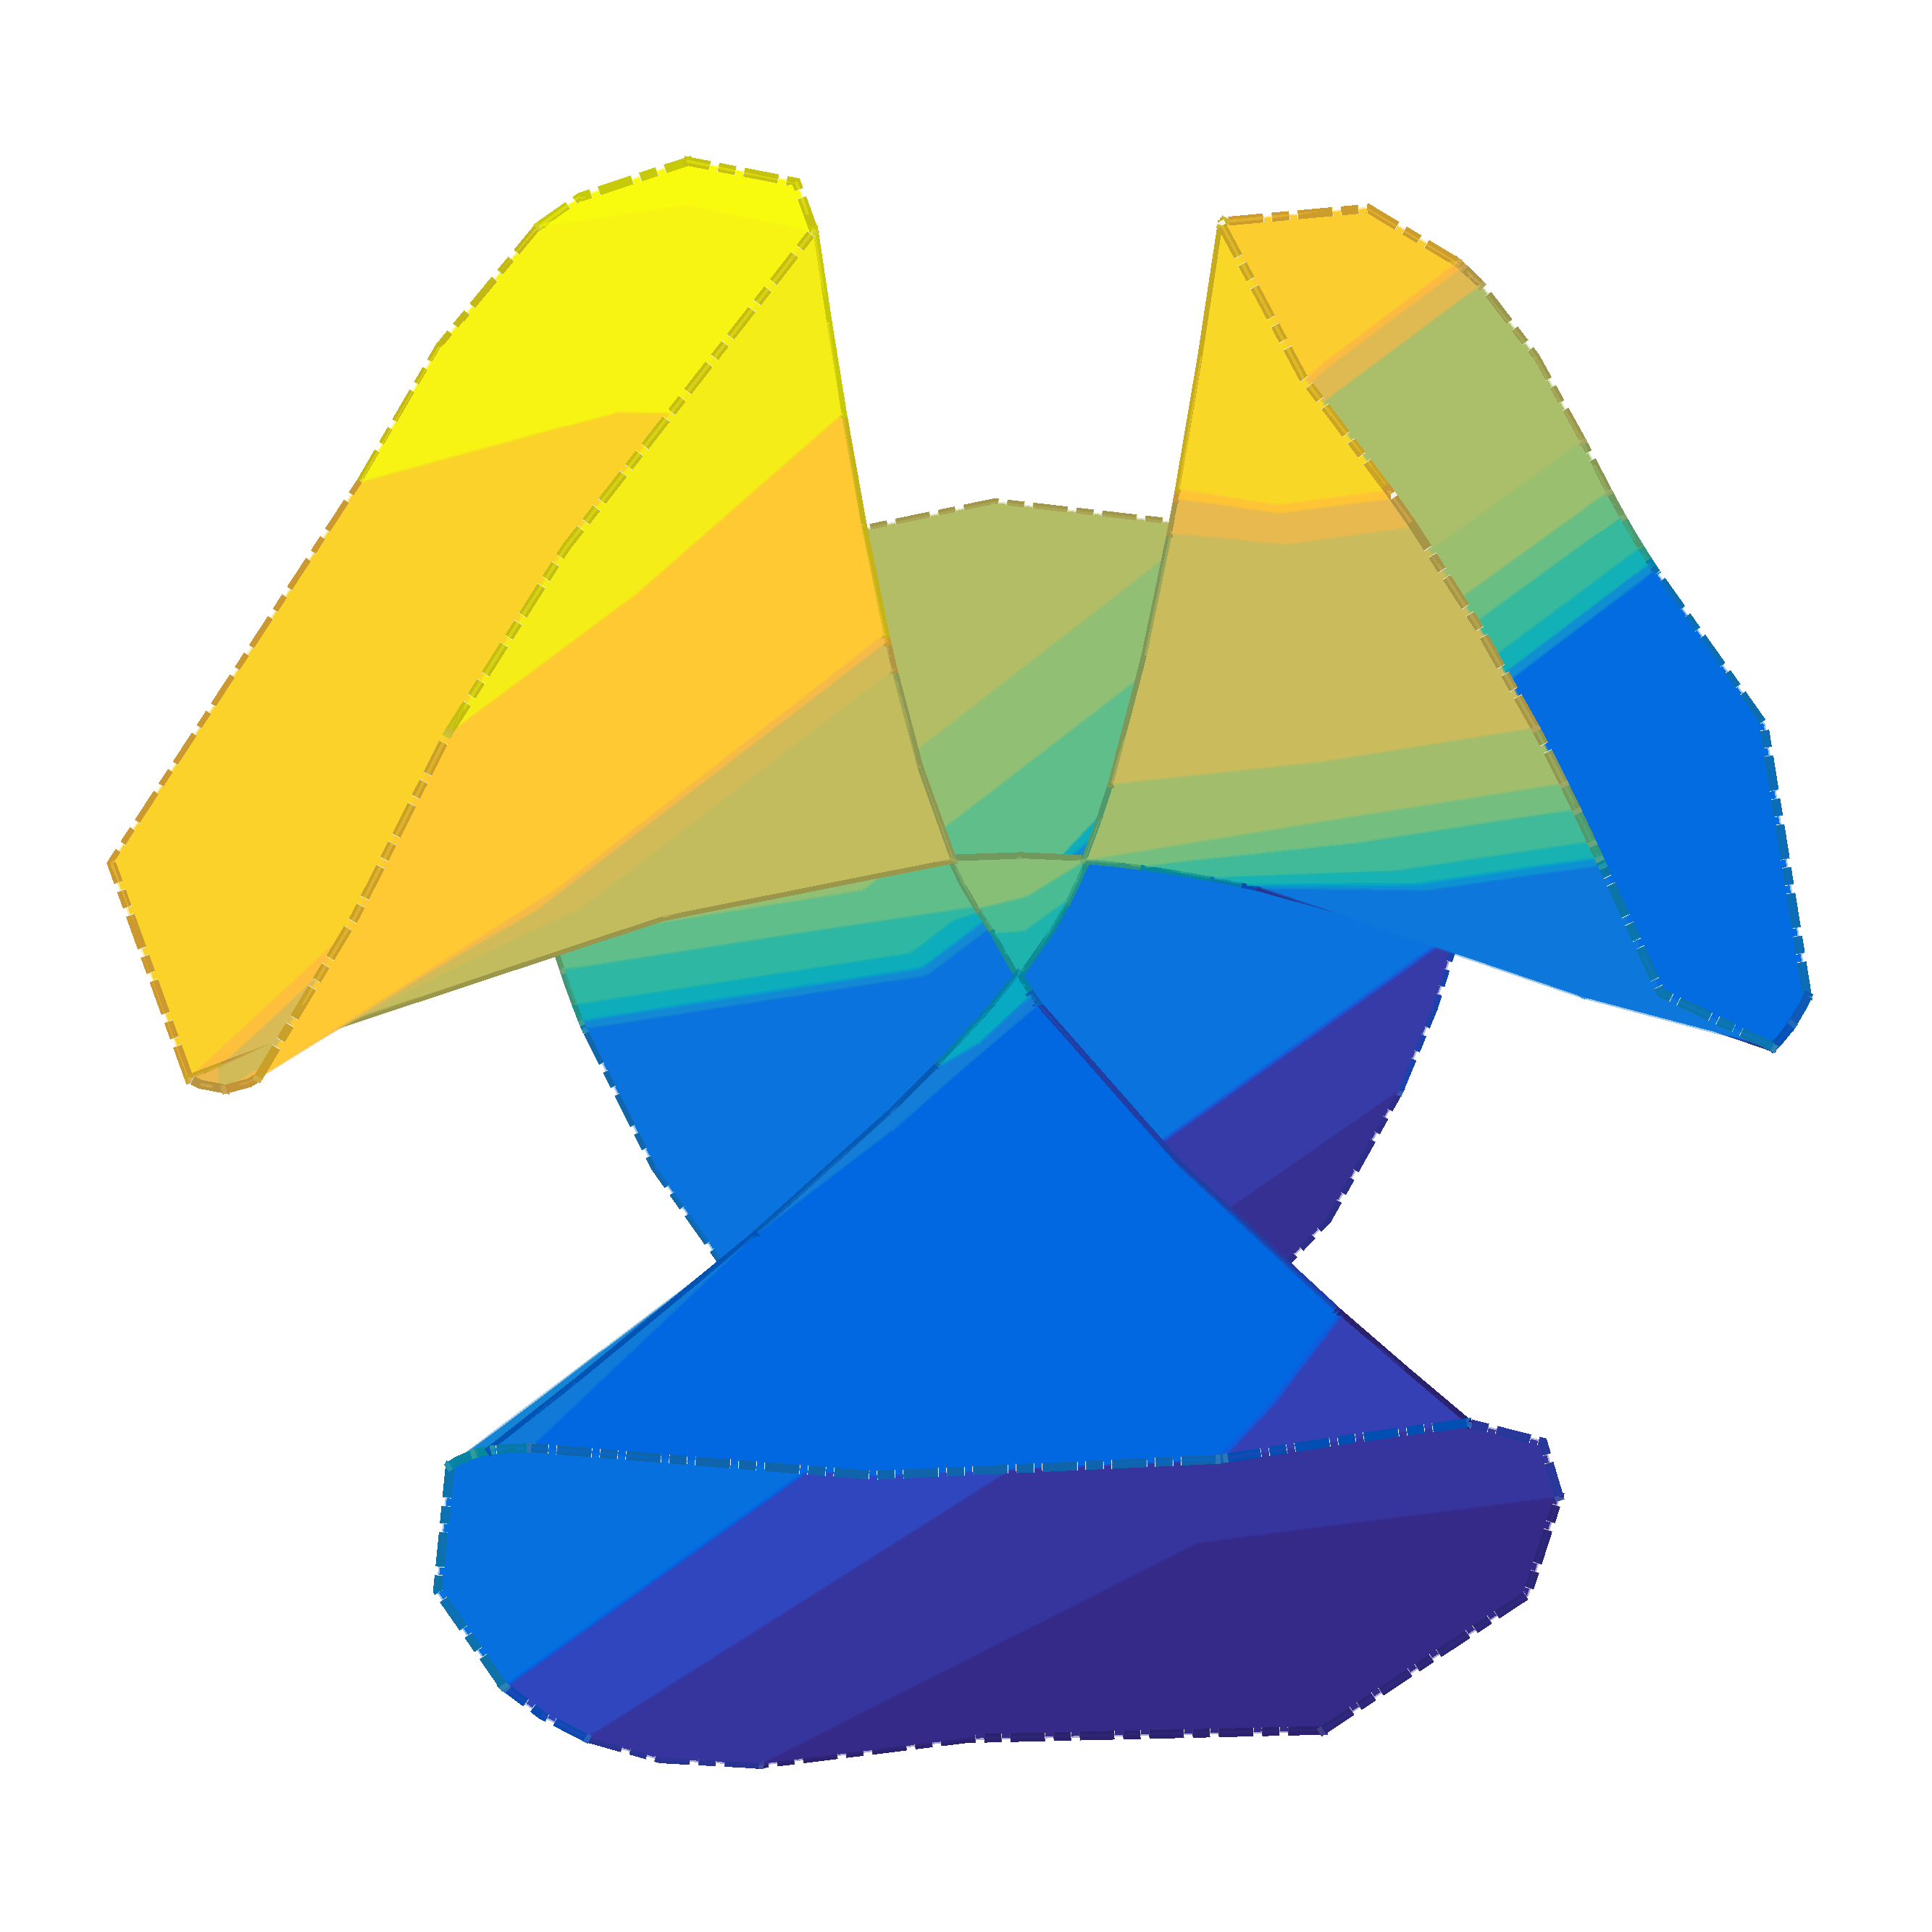
\includegraphics[width = 11cm, height = 5cm]{CayleyCubic.png}
\end{figure}


\section{Compilation and Installation}
\label{sec:installation}

\subsection{Installation}
Before installing Bertini\_real, you must first be sure to have several libraries and dependencies that the software requires. \par
First, you must install Bertini (as a library).  The Bertini source code can be found \newline at \url{https://bertini.nd.edu/download.html}. Download the Bertini source code using the \texttt{./configure} \&\& \texttt{make} \&\& \texttt{make install} process.  Bertini itself has the following dependencies: a C++ compiler capable of the C++ 11 standard, an MPI (such as MPICH2), Boost $>$= 1.53, MPFR, and GMP. Instructions specifically for mac users are listed below. If on Linux, use the package manager provided (e.g. apt-get). Unfortunately, Windows users are unsupported at this time, except possibly through Cygwin or a virtual machine. If interested in porting Bertini and Bertini\_real to windows, please contact Dr. Brake at dbrake@nd.edu. Bertini\_real also is dependent on MATLAB. Once Bertini and all the necessary dependencies are installed, navigate to the directory containing Bertini\_real and install Bertini\_real via the \texttt{./configure} \&\& \texttt{make} \&\& \texttt{make install} process. \par
\subsection{Installation of Bertini/Bertini\_real on macintosh}

\indent If you are using a mac, we encourage the use of Homebrew (\url{http://brew.sh}) to install these packages. After installing Homebrew itself, installing the previously listed dependencies becomes simple. In terminal,  type \texttt{brew search \_\_\_\_} to list packages related to \_\_\_\_, where \_\_\_\_ is your search (for example, GMP, Boost, or MPICH2). To download via Homebrew, type in terminal \texttt{brew install \_\_\_\_}.


\clearpage
\section{Using Bertini\_Real}
\label{sec:running}

\subsection{Input File}
Running Bertini\_real starts with creating a valid input file for Bertini to run on.  With regards to Bertini\_real, the important point about the input file is the tracktype setting. The input file must have the following configuration setting: \texttt{tracktype:1}, which specifies a basic positive dimensional run for Bertini. Using this setting allows for the necessary output files to be produced for Bertini\_real to run. For more information on the structure and syntax of input files, please see the Bertini User Manual  (\url{https://bertini.nd.edu/BertiniUsersManual.pdf}).

\subsection{Running Bertini}
Once a valid input file has been created, Bertini can be run on the input file. This simply amounts to typing on the command line: \texttt{bertini filename}. If the input file is named \texttt{input}, then no filename is needed. Running Bertini will produce the witness points, the points on the curve or surface, which Bertini\_real will later track. Running Bertini also produces the witness linears which are used in the regeneration and slicing steps of the algorithm. The necessary file for Bertini\_real is called \texttt{witness\_data}. 


\subsection{Running Bertini\_real}
The next step is to call Bertini\_real on the command line. This is done simply by calling \texttt{bertini\_real} from the command line. If the input file is called anything other than \texttt{input}, than the \texttt{-input} or \texttt{-i} option followed by the filename must be used (more information below). Bertini\_real uses the tracker options for Bertini, which are set at the top of the input file. We suggest the following configuration options in the input file for Bertini\_real: sharperndigits $>$ 0, imagthreshold $\sim$ 1e-5. Other options can improve performance and tighten up the produced decomposition.
It is important to note that for Bertini\_real to run, the MATLAB executable must be on the path

\subsection{Command Line Options}
Below are the command line options for Bertini\_real. These are placed after the initial \texttt{bertini\_real} command. Each command starts with a single dash, and any required arguments should be placed after. For example, if the user wanted to run Bertini\_real decomposing a specific component, he or she would type: \texttt{bertini\_real -component x}, where x is the integer index of the component to decompose.


\begin {itemize}
\item \texttt{-component}, \texttt{-comp}, or \texttt{-c} \newline Required argument is the integer index of the component for Bertini\_real to decompose (e.g \texttt{-component 1})
\item \texttt{-debug} \newline If used, program will pause for 30 seconds before running for debugging purposes. No required argument.
\item \texttt{-dim} or \texttt{-d} \newline Required argument is the target dimension for Bertini\_real to shoot for
\item \texttt{-gammatrick} or \texttt{-g} \newline Indicator for whether Bertini\_real should use the gamma trick in a particular solver. Required argument is either 1 (if you'd like Bertini\_real to use the gamma trick) or 0 (if not).
\item \texttt{-help}  or \texttt{-h} \newline Displays a help message containing the version of Bertini\_real, where Bertini\_real can be found online, support information, and finally the command line options.
\item \texttt{-input}  or \texttt {-i} \newline Used if input file is named something other than `input'. Required argument is the filename. 
\item \texttt{-mode} or \texttt{-m} \newline Sets the mode of Bertini\_real to be used. Required argument is the mode of operation, and there are currently two valid modes (\texttt{bertini\_real} and \texttt{crit}). \texttt{bertini\_real} is the default mode. 
\item \texttt{-nostifle} or \texttt{-ns} \newline If used, screen output will not be stifled. No required argument
\item \texttt{-nomerge} or \texttt{-nm} \newline Indicates that Bertini\_real should not merge ends. No required argument.
\item \texttt{-output}, \texttt{-out}, or \texttt{-o} \newline Required argument is the name of the output directory.
\item \texttt{-projection}, \texttt{-pi}, or \texttt{-p} \newline Indicator for whether to read the projection from a file, rather than randomly choose it. Required argument is the filename. 
\item \texttt{-quick} or \texttt{-q} \newline Sets the level of quickness for the solver. The quicker the solver, the less robust. 
 \comment{              Not sure the difference between setting quick\_run value to be 1 or 2 via -quick and -veryquick}
\item \texttt{-veryquick} or \texttt{-vq} \newline Sets the level of quickness for the solver. The quicker the solver, the less robust. 
\item \texttt{-sphere} or \texttt{-s} \newline Sets indicator that Bertini\_real should use sphere created by user rather than just compute sphere. Required argument is the name of the file for Bertini\_real to read
\item \texttt{-verb} \newline Required argument is the level of the verbosity you'd like to set.
\item \texttt{-version} or \texttt{-v} \newline Displays the version of Bertini\_real running on your computer. Has no required argument. 
\end{itemize}



\section{Troubleshooting}

\section{Visualization}
After running Bertini\_real, the output results can be visualized in MATLAB. First, open MATLAB and call \texttt{gather\_br\_samples}. This parses the output from Bertini\_real into a .mat file. Then, call \texttt{bertini\_real\_plotter}, which creates a handle class object and facilitates selection of parts of the decomposition to view. There are many options, all of which are documents and displayed via \texttt{help bertini\_real\_plotter} in MATLAB. To run bertini\_real\_plotter with a specific option, type in MATLAB \texttt{bertini\_real\_plotter(`option', `option\_argument')}, where the option\_argument will vary depending on the option you decide to alter. The options are listed below. 
\subsection{Visualization options}
\begin{itemize}

\item \texttt{`autosave'} \newline
By default, the autosave option is on. Thus, the autosave option can be used if you do not want a figure to be automatically saved to the working directory upon creation. Either `false' or 0 can be used to disable autosave. (e.g. \texttt{bertini\_real\_plotter(`autosave', `false')}).

\item \texttt{`colormap'} \newline
Users can alter the colormap used by MATLAB with the `colormap' option by providing a handle to another color map. A full list of built-in colormaps can be found online on the MATLAB help site. \newline (e.g. Using the summer colormap: \texttt{bertini\_real\_plotter(`colormap', @summer)})

\item \texttt{`curve'} or \texttt{`curves'} \newline
By default, the figure created by \texttt{bertini\_real\_plotter} allows the user to display raw curves on the figure. The user can disable this option by setting `curve'  or `curves' to false. To disable curves, the user can use `n', `no', `none', `false', and 0. \newline (e.g \texttt{bertini\_real\_plotter(`curve', `false')})

\item \texttt{`faces'} \newline
By default, the figure created in MATLAB will show both the raw curves and faces. By setting `faces' to false, only the option to display the raw curves will be given. To disable faces, you can use `n', `no', `none', `false', and 0. \newline (e.g \texttt{bertini\_real\_plotter(`faces', 'none')})

\item \texttt{`filename'} or \texttt{`file'} \newline
By default, \texttt{bertini\_real\_plotter} looks for any .mat file that begins with \texttt{BRinfo} . If more than one of those files exists, it looks for the most recent one and uses that in the visualization. If you'd like to specify a specific file to visualize, whether it's an older file from a previous run of \texttt{gather\_br\_samples} a file with a different filename structure alltogether, the filename option allows this. \newline (e.g. \texttt{bertini\_real\_plotter(`filename', `Example\_File\_Name.mat')})

\item \texttt{`labels'} \newline 
By default, the figure created by \texttt{bertini\_real\_plotter} allows the user to apply labels to the figure upon creation. If you would like to disable this option, you can use the labels option with any of the following arguments `n' ,`no', `none', `false', or 0. \newline (e.g. \texttt{bertini\_real\_plotter(`labels', `none')}).  

\item \texttt{`linestyle'} \newline 
Used to change the line style of lines in the MATLAB figure. Options include: `-' (solid line), `--' (dashed line), `:' (dotted line), and `-.' (dash-dot line). \newline (e.g. \texttt{bertini\_real\_plotter(`linestyle', `:')})

\item \texttt{`monocolor'} or \texttt{`mono'} \newline
Used to create a mono-color figure. Required argument is either a RGB triple (row vector with three columns with each entry ranging from zero to one) or one of the following options: `r' (red), `g' (green) `b' (blue),  `m' (magenta), `c' (cyan) `y' (yellow), and `k' (black). For example, creating a red-only figure would be done by typing in MATLAB: \texttt{bertini\_real\_plotter(`mono', `r')}. By default the mono-color option is off.


\item \texttt{`proj'} 
\comment{ 	Unsure of what proj does}


\item \texttt{`vertices'} or \texttt{`vert'} \newline
By default, the figure created in MATLAB will allow the user to place vertex markers and labels on the figure. Setting `vertices' to false disables this option. To disable vertices, you can use `n', `no', `none', `false', and 0. \newline (e.g \texttt{bertini\_real\_plotter(`vertices', 0)})


\end{itemize}

\section{3D Printing}

\clearpage

\appendix
\section{Output Formats}


\subsection{.curve}


(num\_variables total) num\_vertices num\_edges \\
num\_V0 num\_V1 num\_midpts num\_newpts \\

indices of V0  \\
indices of V1  \\
indices of midpoints \\
indices of added\_points

projection excluding the homogeneous 0 coordinate.\\

\File{Example C.curve file. }{C.curve}{C.curve}

\subsection{.edge}


\subsection{.vert}




%\ifx\standalonemode\undefined
%
%\else
%	\begin{singlespace}
%	\bibliographystyle{ieeetr}
%	\bibliography{bibliobiblioparama}
%	\end{singlespace}
%	
%	\begin{singlespace}
%	\printindex
%	\end{singlespace}
%\fi

\end{document}